\documentclass[11pt,a4paper]{article}

\usepackage[left=2cm,text={17cm,24cm},top=3cm]{geometry}
\usepackage[english]{babel}
\usepackage[utf8]{inputenc}
\usepackage[T1]{fontenc}
\usepackage{indentfirst}
\usepackage{hyperref}
\usepackage{float}
\usepackage{siunitx}

\usepackage{textcomp}
\newcommand{\tilda}{\raisebox{0.5ex}{\texttildelow}}

% URL
\usepackage{url}
\def\UrlBreaks{\do\/\do-}
\usepackage{breakurl}

% IMG
\usepackage{graphicx}
\graphicspath{{.}}

\usepackage{etoolbox}
\patchcmd{\thebibliography}{\section*{\refname}}{}{}{}

% #################################################################################################
\begin{document}
% #################################################################################################


% #################################################################################################
% TITLEPAGE
\begin{titlepage}
    \begin{center}
        \Huge
        \textsc{
            Faculty of Information Technology\\
            Brno University of Technology
        }
        \vspace{80px}
        \begin{figure}[!h]
            \centering
            
\includegraphics[scale=0.3]{img/vutbr-fit-logo.eps}
        \end{figure}
        \\[15mm]
        \Huge{
            \textbf{
                SEN
            }
        }
        \\[1.5mm]
        \huge{
            \textbf{
                Intelligent Sensors
            }
        }
        \\[2.5em]
        \LARGE{
            \textbf{
                Commissioning Heartbeat Sensor and Comparison\\
                Against Oximeter
            }
        }
        \vfill
    \end{center}
        \Large{
            \hfill\\
            Jiří Záleský (xzales12)\\
            Adrián Tóth (xtotha01)\hfill \today
        }

\end{titlepage}


% #################################################################################################
% CONTENT


\setlength{\parskip}{0pt}
\hypersetup{hidelinks}\tableofcontents
\setlength{\parskip}{0pt}

\newpage

\section{Project}

The aim of this project is to comission a heart beat sensor. Within the project, there will be done several measurements, which will be later compared with the results of a valid device - oximeter. Prof. Ing., Dipl.-Ing. Martin Drahanský, Ph.D\footnote{\href{http://www.fit.vutbr.cz/~drahan/}{www.fit.vutbr.cz/{\tilda}drahan}} is the project supervisor.

\section{Abstract}

The aim of this project is to demonstrate a method of measuring heart beat via infrared light. The upcoming sections will describe further requirements to achieve the right functionality. The results of measurement were compared with a valid heart beat sensor, which measured heart beat in other way than the infrared method.

\section{Introduction}

The infrared light has a key role in this project. The infrared LED represents a main source of infrared rays which are sent in a direction to phototransistor. These rays may be affected by any kind of object representing a blockade in the way to the phototransistor. Using a finger as a rays blockade, the rays are affected not only by the finger itself, but also by the blood in the finger. As the heart is pulsing inside of the person's body, the blood pressure is different inside of the finger's veins, which has also a great impact on the rays. The emitted rays from the finger are detected by the phototransistor that produces a precise values. Based on these values, there is a possibility to detect heart beat. This method of measurement is shown in Figure \ref{fig:method}.

\begin{figure}[H]
    \centering
    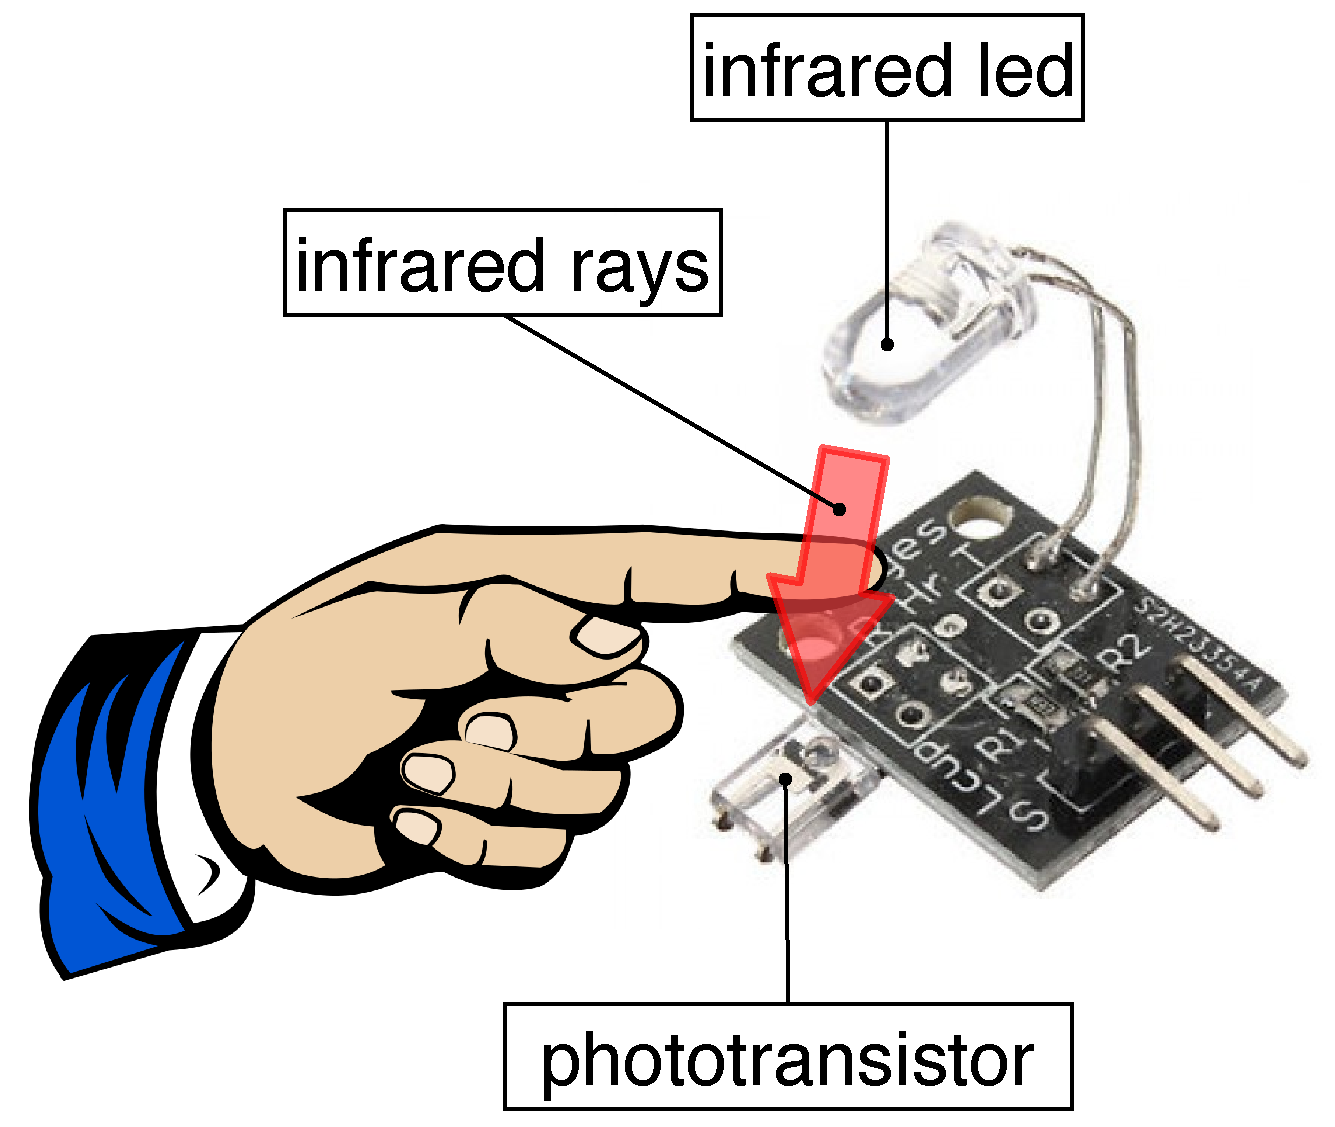
\includegraphics[scale=0.4]{img/infrared_method.pdf}
    \caption{Method of infrared heart beat measurement.}
    \label{fig:method}
\end{figure}

\newpage

The necessary facilities for the implementation of the project were:\\[-1.5em]
\begin{itemize}
    \item Device shown in Figure \ref{fig:oldplatform}.\\[-2em]
        \begin{figure}[H]
            \centering
            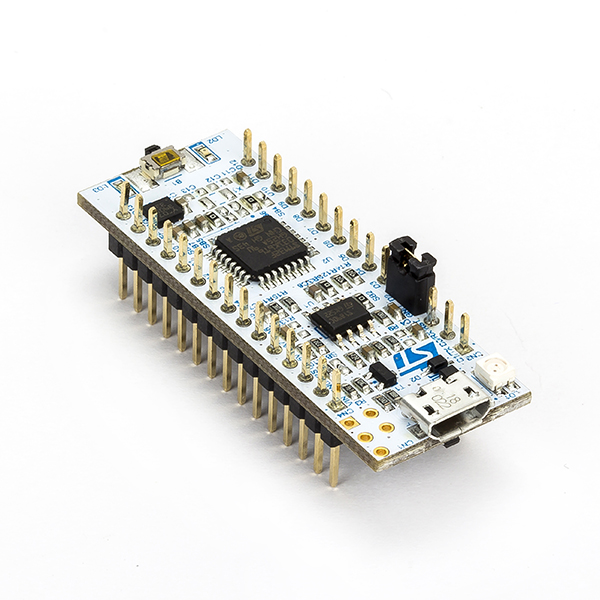
\includegraphics[scale=1.4]{img/device-old.jpg}
            \caption{STM32 Nucleo board~\cite{IMG-DEVICE-OLD}.}
            \label{fig:oldplatform}
        \end{figure}
        \hfill\\[-17mm]
    \item Sensor shown in Figure \ref{fig:senzor1}.
        \begin{figure}[H]
            \centering
            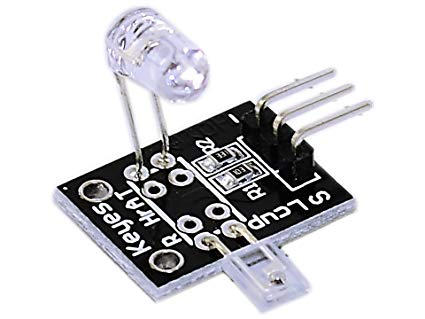
\includegraphics[scale=0.3]{img/sensor1.jpg}
            \caption{Keyes KY-039 Finger Heartbeat Detection Sensor~\cite{IMG-SENSOR-1}.}
            \label{fig:senzor1}
        \end{figure}
        \hfill\\[-18mm]
    \item Three female--to--female jumper wires.\\[-2.5mm]
\end{itemize}

After we received the devices, we faced a lot of problems. The main device representing the basic platform was not working properly so we had to ask for a new one. Later, the main device (shown in Figure \ref{fig:oldplatform}) was replaced to a new one (see Figure \ref{fig:platform1}) due to wrong functionality by the technical assistant of the project - Ing. Tomáš Goldmann\footnote{\href{http://www.fit.vutbr.cz/~igoldmann/}{www.fit.vutbr.cz/{\tilda}igoldmann}}.

\newpage

\begin{figure}[H]
    \centering
    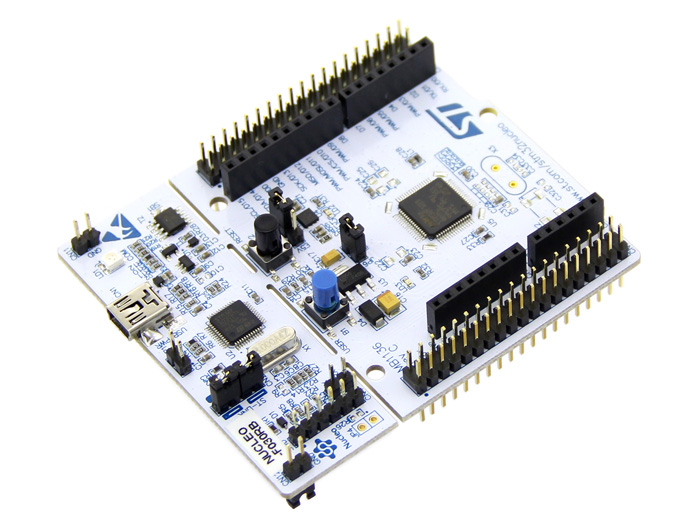
\includegraphics[scale=0.4]{img/device1.jpg}
    \caption{STM32 Nucleo board~\cite{IMG-DEVICE-1}.}
    \label{fig:platform1}
\end{figure}

\indent The device shown in Figure \ref{fig:platform1} - NUCLEO-F030R8~\cite{PLATFORM}, was the main platform for the project. The device was equipped with a STM32F030R8~\cite{MCU} microcontroller unit (MCU), which was designed and made to be suitable for a wide range of applications. MCU includes a set of peripherals through which it communicates with other devices such as the sensor shown in Figure \ref{fig:senzor1}. To create a communication pipeline, these units must be connected to each other via jumper wires. Wires provide a connection between the pins of units and so the pins have to be configured correctly.

\section{Setup}

Firstly, the components must be connected to each other in a right way. Sensor, as a slave component shown in Figure \ref{fig:senzor2wires}, is connected to the main device (master component). These two units are connected via 3 jumper wires to the corresponding pins. The Figure \ref{fig:device2wires} and \ref{fig:senzor2wires} have three common marked pins: \textit{GND} (orange), \textit{5V} (yellow), \textit{PA0} and \textit{S} (green); by which they are connected together. \textit{PA0} indicates an analog input pin to the master component. A precise description of all the necessary pins is shown in Figure \ref{fig:legend}.

\begin{figure}[H]
    \centering
    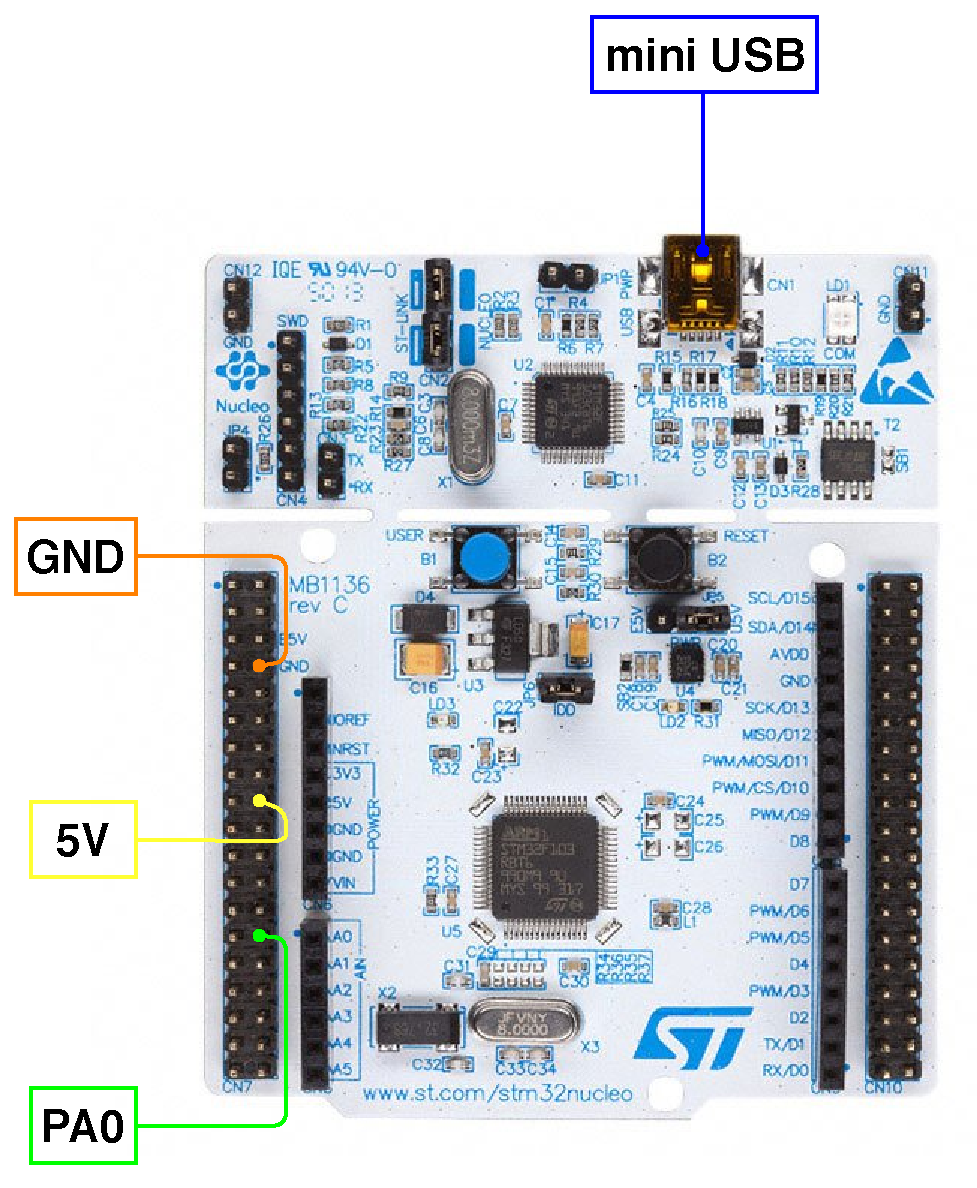
\includegraphics[scale=0.5]{img/device2-wires.pdf}
    \caption{NUCLEO-F030R8~\cite{IMG-DEVICE-2} connection scheme.}
    \label{fig:device2wires}
\end{figure}

\begin{figure}[H]
    \centering
    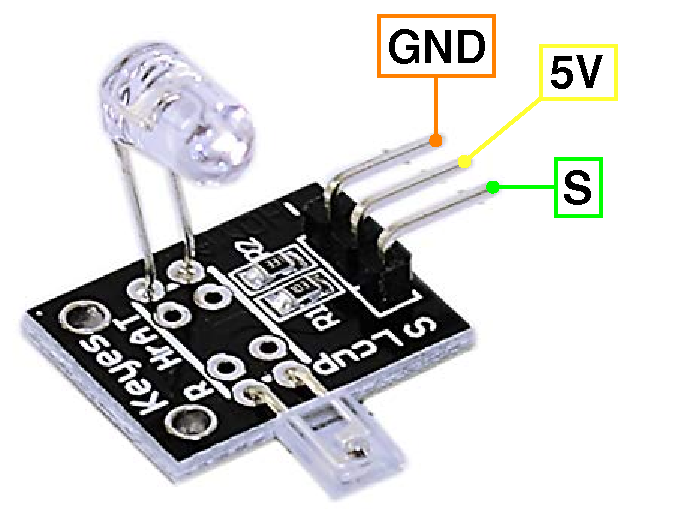
\includegraphics[scale=0.5]{img/sensor1-wires.pdf}
    \caption{Keyes KY-039~\cite{IMG-SENSOR-1} connection scheme relating to Figure \ref{fig:device2wires}.}
    \label{fig:senzor2wires}
\end{figure}

\begin{figure}[H]
    \begin{center}
        \begin{tabular}{|r|l|}
            \hline
            \textbf{S}        & sensor output \\
            \hline
            \textbf{B1}       & button 1 \\
            \hline
            \textbf{B2}       & button 2 \\
            \hline
            \textbf{LD2}      & LED 2 \\
            \hline
            \textbf{GND}      & ground \\
            \hline
            \textbf{5V}       & 5 volt voltage supply \\
            \hline
            \textbf{PA0}      & pin PA0 \\
            \hline
            \textbf{mini USB} & mini USB port \\
            \hline
        \end{tabular}
    \end{center}
    \caption{Explanatory notes.}
    \label{fig:legend}
\end{figure}

A connection scheme of the devices is shown in Figure \ref{fig:old_con_scheme}. After the devices were correctly connected and attached to the computer via mini USB port (see Figure \ref{fig:connection}), they were ready to be programmed.

\begin{figure}[H]
    \centering
    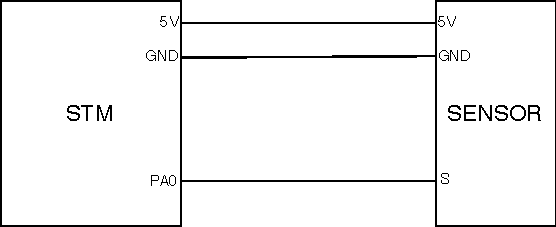
\includegraphics[scale=1.4]{img/old_con_scheme.pdf}
    \caption{Device connection scheme.}
    \label{fig:old_con_scheme}
\end{figure}

\begin{figure}[H]
    \centering
    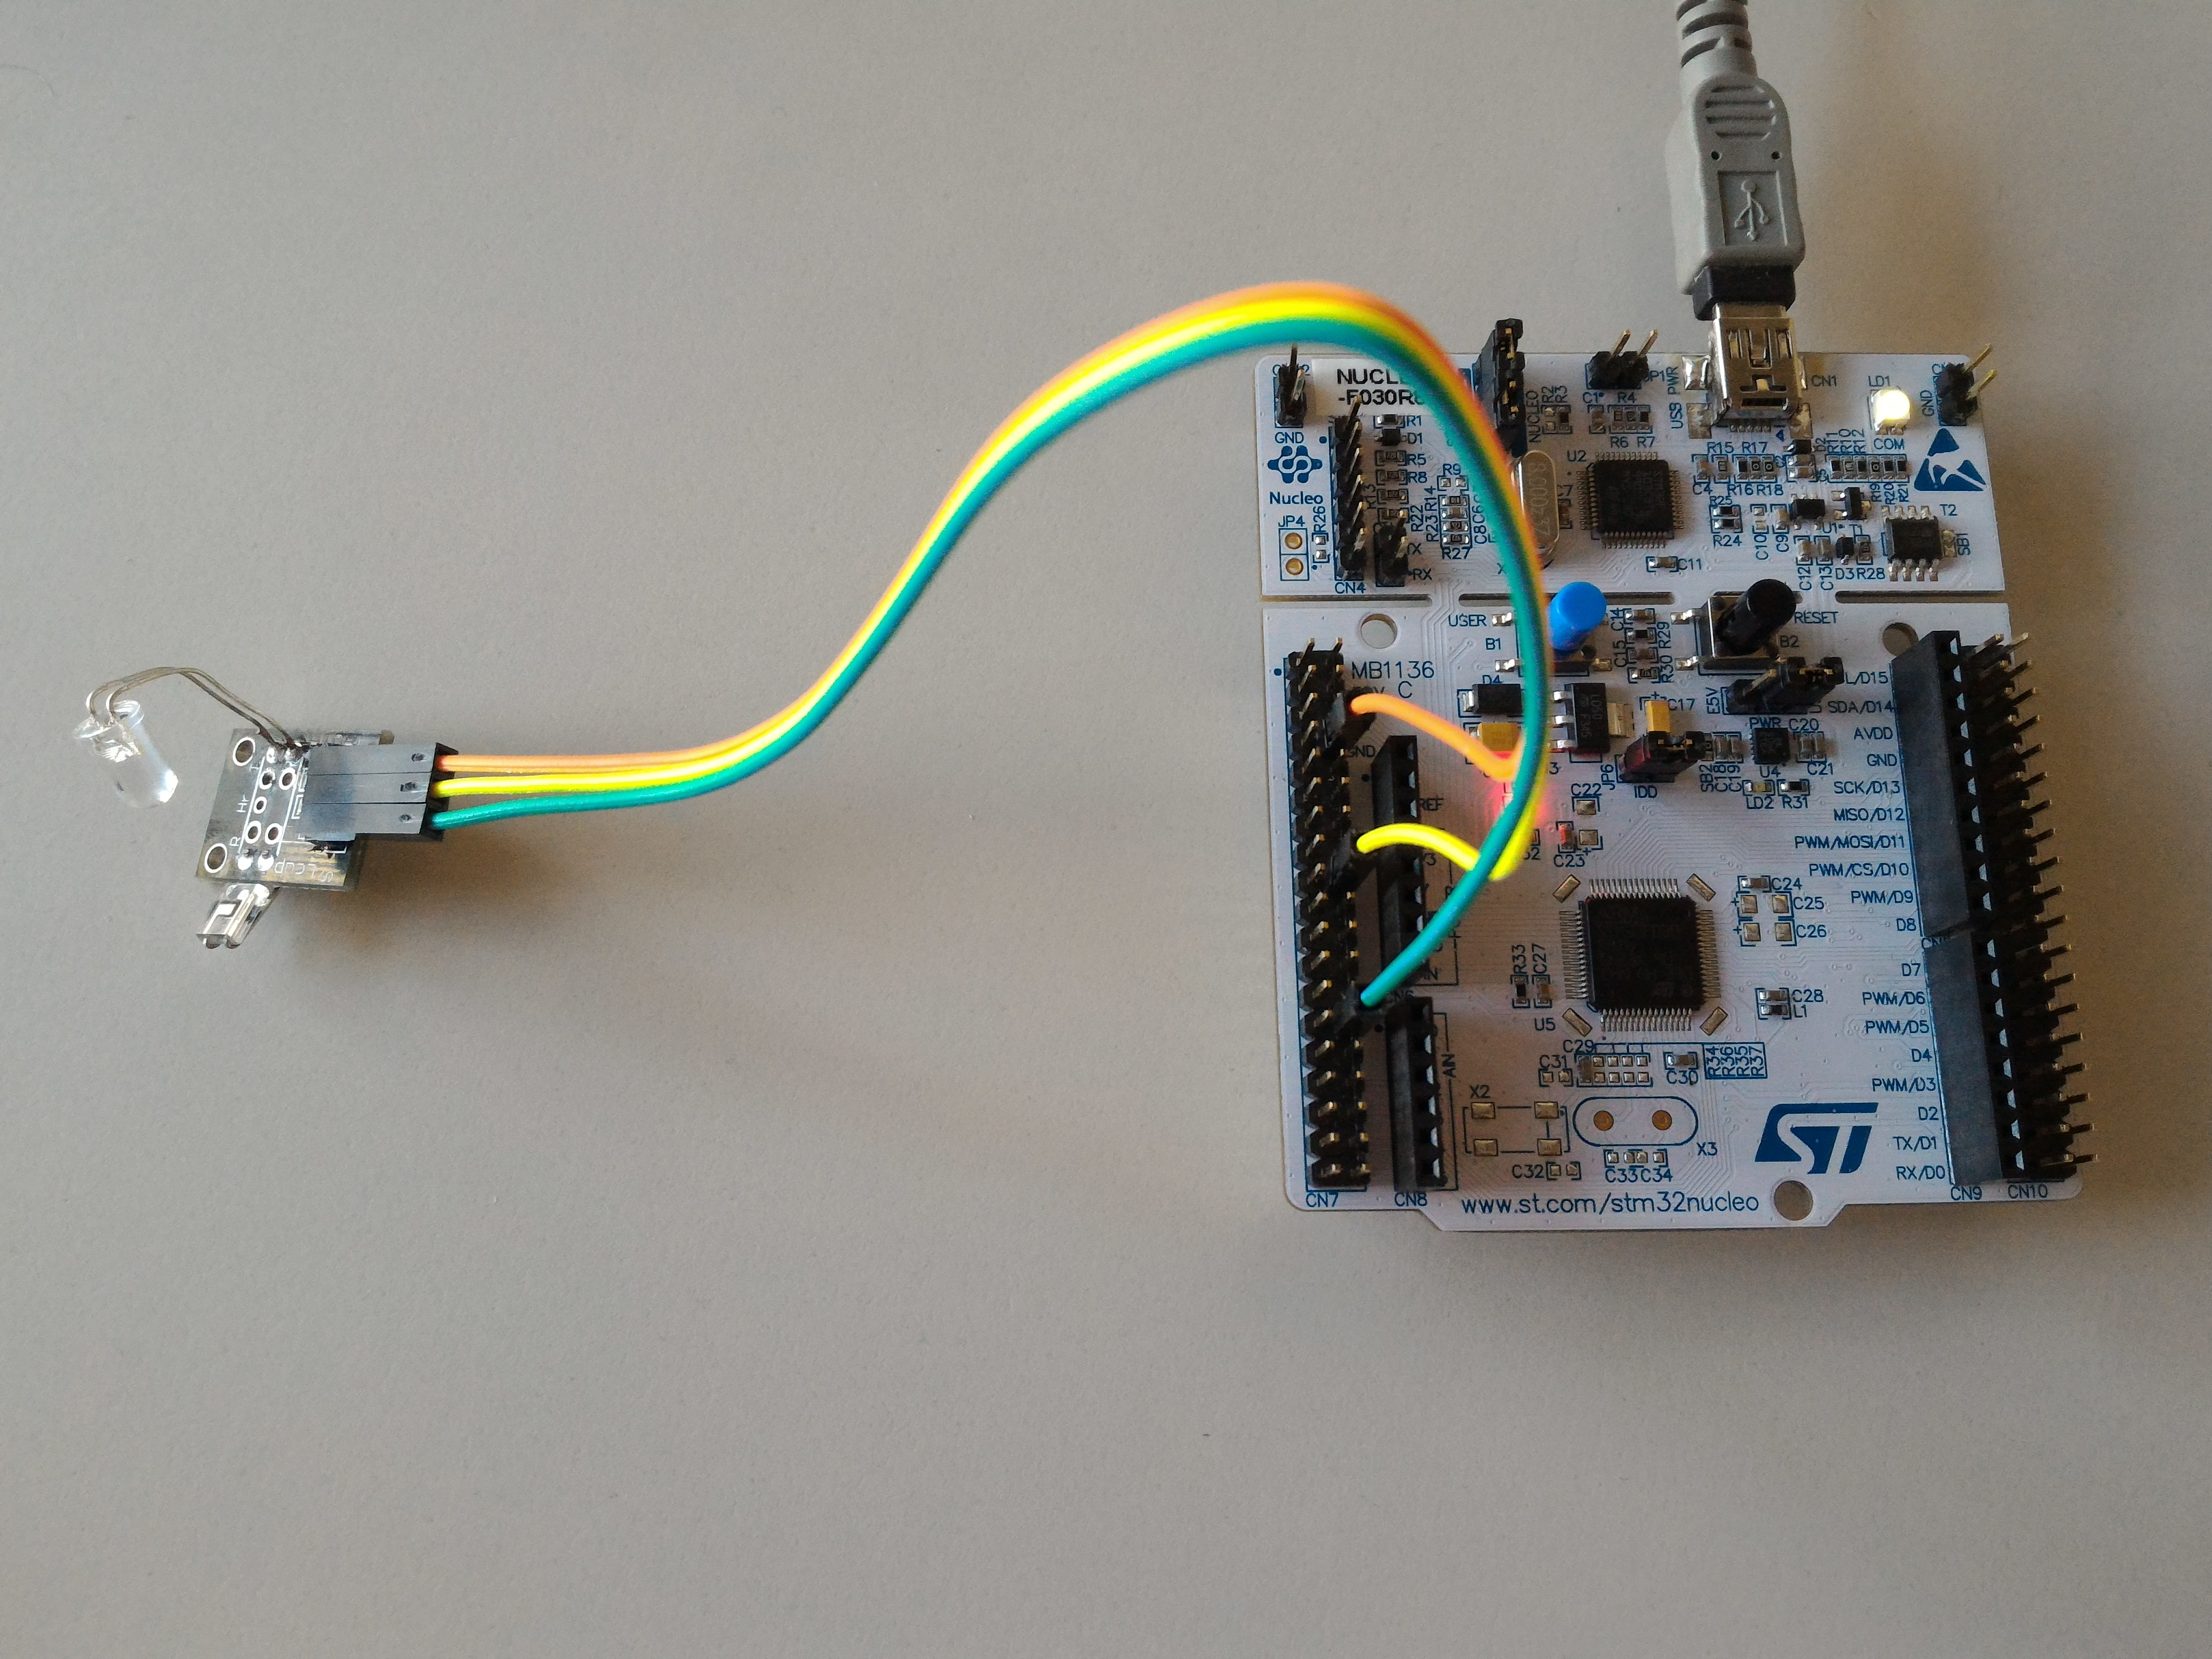
\includegraphics[scale=0.1]{img/setup1.jpg}
    \caption{Correct connection of devices.}
    \label{fig:connection}
\end{figure}

As we were working on the implementation part of the project, there was a measurement anomaly. The results were affected by different input voltage on the pin. We asked for an advice from the technical assistant. He has recommended us a different device connection which is shown in Figure \ref{fig:new_con_scheme}. He suggested to use a protoboard with two 10k\si{\ohm} resistors and a few additional connection wires.

\begin{figure}[H]
    \centering
    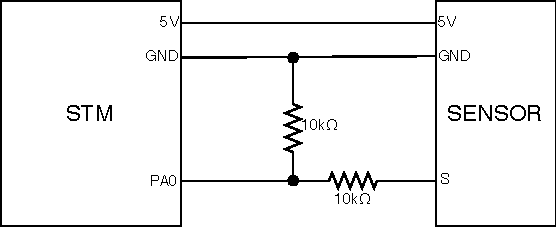
\includegraphics[scale=1.4]{img/new_con_scheme.pdf}
    \caption{New device connection scheme.}
    \label{fig:new_con_scheme}
\end{figure}

The devices have been reconnected based on the given advice, which is shown in Figure \ref{fig:new_dev_con}. This setup was the proper one where the values have not been affected by voltage.

\begin{figure}[H]
    \centering
    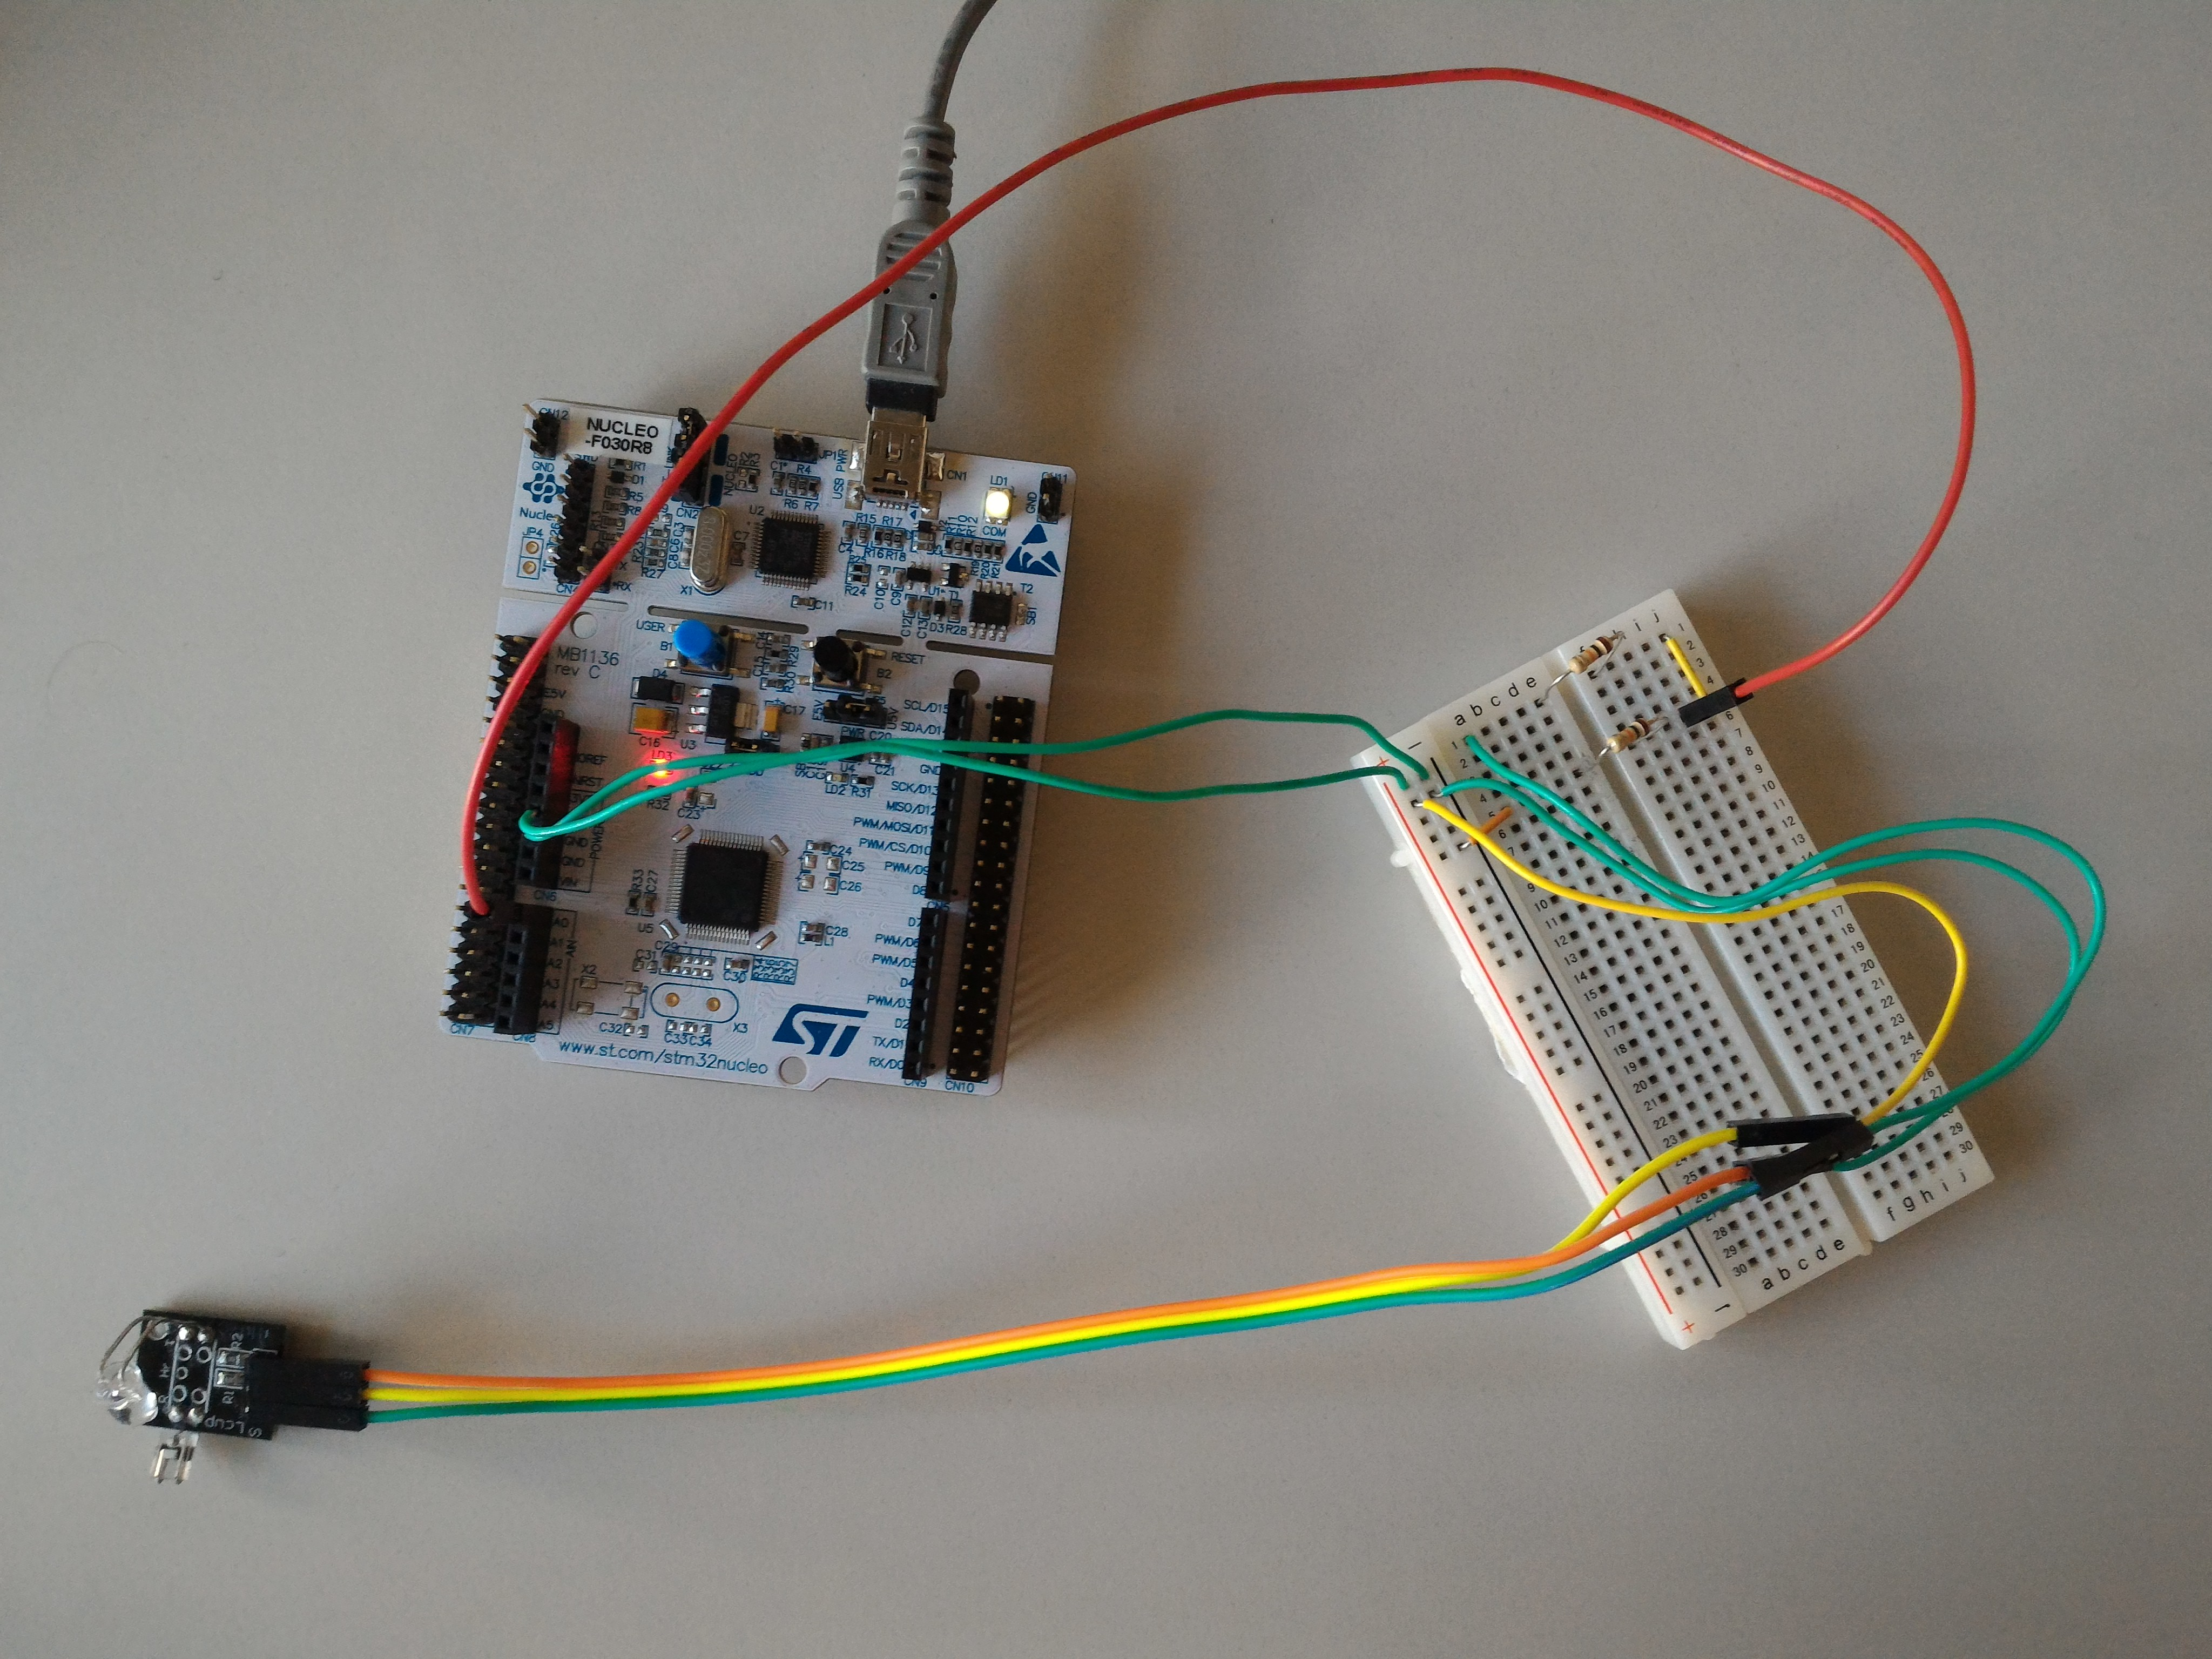
\includegraphics[scale=0.1]{img/setup2.jpg}
    \caption{New connection of devices.}
    \label{fig:new_dev_con}
\end{figure}

\newpage

\section{Implementation}
The implementation is based on an algorithm~\cite{SENSOR}, which detects deviation in a set of incoming values from the sensor. The values, incoming as a sequence of measurements, contain a few values that have a certain deviation what indicates the pulse. This is the deviation on which basis we can calculate the hear beat per minutes also know as beats per minute (BPM). The program will light up a LED (see LD2 in Figure \ref{fig:device2wires}) on each beat. The BPM is calculated from one period - the time between two hear beats. No history is used for the calculations.\\

Algorithm itself is a little bit complicated due to moving interval of incoming values. The finger position significantly affects the value interval but do not have any impact on the deviation between the values. To detect a deviation, it is necessary to keep a previous value from the sequence. A comparison action is provided which will determine divergence between the values. If this action will establish the deviation as large enough, this value will be determined as a beat at that moment.\\

The precision of the algorithm depends on the device configuration and its precision. It is nearly impossible to make a universal algorithm which can determine heart beat on inaccurate values. The more accurate the sensor values, the more precise the results. As an accuracy factor we can count with a finger motion that has the biggest impact on the BPM calculations. By examining the sensor, we can see that the phototransistor is not sealed into rubber. This fact indicates, that the sensor is receiving external infrared rays from the surrounding area. We can assume that the surrounding area can influence the results.

\section{Conclusion}
...

\newpage %#########################################################################################

\section{Appendix}

\begin{figure}[H]
    \begin{center}
        \begin{tabular}{|l|c|}
            \hline
            \textbf{Name} & \textbf{Value} \\
            \hline\hline
            n1 & v1 \\\hline
            n2 & v2 \\\hline
            n3 & v3 \\\hline
        \end{tabular}
    \end{center}
    \caption{Table of measurements.}
    \label{fig:measurements}
\end{figure}

\newpage %#########################################################################################

\section{References}
\bibliographystyle{englishiso}
\begin{flushleft}
    \bibliography{quotation}
\end{flushleft}


% #################################################################################################
\end{document}
% #################################################################################################
